\documentclass[10pt,a4paper]{article}
\usepackage[utf8]{inputenc}
\usepackage[spanish]{babel}
\usepackage{amsmath}
\usepackage{amsfonts}
\usepackage{amssymb}
\usepackage{graphicx}

% Default fixed font does not support bold face
\DeclareFixedFont{\ttb}{T1}{txtt}{bx}{n}{6} % for bold
\DeclareFixedFont{\ttm}{T1}{txtt}{m}{n}{6}  % for normal

% Custom colors
\usepackage{color}
\definecolor{deepblue}{rgb}{0,0,0.5}
\definecolor{deepred}{rgb}{0.6,0,0}
\definecolor{deepgreen}{rgb}{0,0.5,0}

\usepackage{listings}

% Python style for highlighting
\newcommand\pythonstyle{\lstset{
language=Python,
basicstyle=\ttm,
otherkeywords={self},             % Add keywords here
keywordstyle=\ttb\color{deepblue},
emph={MyClass,__init__},          % Custom highlighting
emphstyle=\ttb\color{deepred},    % Custom highlighting style
stringstyle=\color{deepgreen},
frame=tb,                         % Any extra options here
showstringspaces=false            % 
}}


% Python environment
\lstnewenvironment{python}[1][]
{
\pythonstyle
\lstset{#1}
}
{}

% Python for external files
\newcommand\pythonexternal[2][]{{
\pythonstyle
\lstinputlisting[#1]{#2}}}

% Python for inline
\newcommand\pythoninline[1]{{\pythonstyle\lstinline!#1!}}

% Prolog
\lstdefinestyle{myPrologstyle}
{
    language=Prolog,
    basicstyle = \footnotesize\ttfamily\color{blue},
    moredelim = [s][\color{black}]{(}{)},
    literate =
        {:-}{{\textcolor{black}{:-}}}2
        {,}{{\textcolor{black}{,}}}1
        {.}{{\textcolor{black}{.}}}1
}

% XML
\definecolor{maroon}{rgb}{0.5,0,0}
\definecolor{darkgreen}{rgb}{0,0.5,0}
\lstdefinelanguage{XML}
{
  basicstyle=\footnotesize\ttfamily,
  morestring=[s]{"}{"},
  morecomment=[s]{?}{?},
  morecomment=[s]{!--}{--},
  commentstyle=\color{darkgreen},
  moredelim=[s][\color{black}]{>}{<},
  moredelim=[s][\color{red}]{\ }{=},
  stringstyle=\color{blue},
  identifierstyle=\color{maroon}
}

\author{Carlos Manuel Rodríguez Martínez}
\title{Interfaz gráfica para algoritmo solucionador de Sudokus en Prolog}
\begin{document}

\maketitle

\newpage

\tableofcontents

\newpage

\section{Introducción}
Una de las ventajas principales de un lenguaje de programación lógico como Prolog es que permite escribir rutinas con una cantidad mínima de código ya que sólo es necesario especificar las constricciones particulares de cada problema. Siguiendo la filosofía de compactar lo más posible los programas, decidí hacer este proyecto utilizando Python como lenguaje de programación principal y QT como biblioteca de interfaz gráfica.

Además de ser un lenguaje de muy alto nivel, existe la biblioteca PySwip que permite conectar Python con el intérprete de SWI-Prolog. La interfaz es mínima, y junto con las capacidades que ofrece QT para editar fácilmente una interfaz gráfica consideré este lenguaje idóneo para desarrollar este proyecto.

\section{Implementación}
El programa se divide en tres partes, cada una escrita en un lenguaje de programación diferente.

\subsection{Algoritmo solucionador de Sudoku en Prolog}
El algoritmo solucionador está escrito en Prolog y se encuentra como un ejemplo dentro del repositorio del paquete \emph{clpfd}.

\begin{lstlisting}[style=myPrologstyle]
/* Autor original: Markus Triska  (triska@metalevel.at) */

:- use_module(library(clpfd)).

sudoku(Rows) :-
        /* Verifica que el numero de filas sea igual a 9 */
        length(Rows, 9),
        /* Verifica que todas las filas sean del mismo tamano */
	maplist(same_length(Rows), Rows),
        /* Aplana la lista, todo el tablero queda en Vs */
        append(Rows, Vs),
        /* Verifica que todos los elementos de Vs se encuentren en el dominio [0,9] */
	Vs ins 1..9,
        /* Condicion de que todos los elementos de cada fila deben ser distintos */
        maplist(all_distinct, Rows),
        /* Traspone filas para obtener lista de columnas */
        transpose(Rows, Columns),
        /* Condicion de que todos los elementos de cada columna deben ser distintos */
	maplist(all_distinct, Columns),
        /* Unifica Rows con la lista de variables */
        Rows = [As,Bs,Cs,Ds,Es,Fs,Gs,Hs,Is],
        /* Verifica que no se repita ningun digito en cada bloque */
        blocks(As, Bs, Cs), blocks(Ds, Es, Fs), blocks(Gs, Hs, Is).

blocks([N1,N2,N3|Ns1], [N4,N5,N6|Ns2], [N7,N8,N9|Ns3]) :-
        /* Verifica bloques uno por uno recursivamente */
	all_distinct([N1,N2,N3,N4,N5,N6,N7,N8,N9]), blocks(Ns1, Ns2, Ns3).

/* Termina la recursion si todas las listas son vacias */
blocks([], [], []).

/* Resuelve probando diferentes valores para las filas */
solve_sudoku(Board) :- sudoku(Board), maplist(labeling([ff]), Board).
\end{lstlisting}

\subsection{Aplicación principal en Python}
La aplicación principal fue escrita en Python 3 haciendo uso del kit de interfaz gráfica QT, y la biblioteca PySwip que provee una interfaz con el motor de Prolog.

\begin{python}
import sys

# Bibliotecas de interfaz grafica QT
from PySide2.QtUiTools import QUiLoader
from PySide2.QtWidgets import QApplication, QPushButton, QTableWidget, QTableWidgetItem
from PySide2.QtCore import QFile, QObject
from PySide2.QtGui import QColor

# Conexion con Prolog
from pyswip import Prolog

class Form(QObject):
    def __init__(self, ui_file, parent=None):
        super(Form, self).__init__(parent)
        # Open ui file.
        ui_file = QFile(ui_file)
        ui_file.open(QFile.ReadOnly)

        # Carga la interfaz grafica en el objeto Form
        loader = QUiLoader()
        self.window = loader.load(ui_file)
        ui_file.close()

        # Conectar eventos
        solveBtn = self.window.findChild(QPushButton, 'solveBtn')
        solveBtn.clicked.connect(self.ok_handler)

        resetBtn = self.window.findChild(QPushButton, 'resetBtn')
        resetBtn.clicked.connect(self.reset_handler)

        # Localiza objetos que contienen al tablero
        self.topLeft = self.window.findChild(QTableWidget, 'topLeft')
        self.topMiddle = self.window.findChild(QTableWidget, 'topMiddle')
        self.topRight = self.window.findChild(QTableWidget, 'topRight')
        self.middleLeft = self.window.findChild(QTableWidget, 'middleLeft')
        self.middleMiddle = self.window.findChild(QTableWidget, 'middleMiddle')
        self.middleRight = self.window.findChild(QTableWidget, 'middleRight')
        self.bottomLeft = self.window.findChild(QTableWidget, 'bottomLeft')
        self.bottomMiddle = self.window.findChild(QTableWidget, 'bottomMiddle')
        self.bottomRight = self.window.findChild(QTableWidget, 'bottomRight')

        # Comienza el motor de Prolog
        self.prolog = Prolog()
        self.prolog.consult("solver.pl")

        self.window.show()

    # Rutina que se ejecuta cuando el usuario hace click en boton Ok
    def ok_handler(self):
    	# Guarda todos los elementos del tablero en la variable puzzle
        puzzle = [[self.get_value_at(x,y) for y in range(9)] for x in range(9)]
        solution = self.solve_puzzle(puzzle) # Solve puzzle using prolog.

        if solution != False:
            for y in range(9):
                for x in range(9):
                    self.set_value_at(y, x, solution[y][x]) # Fill the board.
            self.window.update()
        else:
            print("Prolog can't solve this board")

    def get_item_value(self, item): # Parse item
        if(hasattr(item, 'text')):
            if item.text() != ' ' and item.text() != '':
                return int(item.text())
            else:
                return 0
        else:
            return 0

    # Obtiene el valor del item en la posicion (x,y). Esto es necesario porque el tablero esta compuesto de 9 widgets.
    def get_value_at(self, x, y):
        horizontal = int(y / 3)
        horizontalIndex = y % 3
        vertical = int(x / 3)
        verticalIndex = x % 3

        if vertical == 0:
            if horizontal == 0:
                return self.get_item_value(self.topLeft.item(verticalIndex, horizontalIndex))
            elif horizontal == 1:
                return self.get_item_value(self.topMiddle.item(verticalIndex, horizontalIndex))
            else:
                return self.get_item_value(self.topRight.item(verticalIndex, horizontalIndex))
        elif vertical == 1:
            if horizontal == 0:
                return self.get_item_value(self.middleLeft.item(verticalIndex, horizontalIndex))
            elif horizontal == 1:
                return self.get_item_value(self.middleMiddle.item(verticalIndex, horizontalIndex))
            else:
                return self.get_item_value(self.middleRight.item(verticalIndex, horizontalIndex))
        else:
            if horizontal == 0:
                return self.get_item_value(self.bottomLeft.item(verticalIndex, horizontalIndex))
            elif horizontal == 1:
                return self.get_item_value(self.bottomMiddle.item(verticalIndex, horizontalIndex))
            else:
                return self.get_item_value(self.bottomRight.item(verticalIndex, horizontalIndex))

    # Colorear item
    def set_item_value(self, item, value):
        if (hasattr(item, 'text')):
            if item.text() != ' ' and item.text() != '':
                item.setText(value)
            else:
                item.setText(value)
                item.setTextColor(QColor("green"))
        else:
            item = QTableWidgetItem(value)
            item.setTextColor(QColor("green"))

    # Coloca el valor del item en la posicion (x,y). Esto es necesario porque el tablero esta compuesto de 9 widgets.
    def set_value_at(self, x, y, value):
        nvalue = str(value)
        newItem = QTableWidgetItem(nvalue)
        current_value = self.get_value_at(x, y)
        if current_value != 0:
            newItem.setTextColor(QColor("green"))

        horizontal = int(y / 3)
        horizontalIndex = y % 3
        vertical = int(x / 3)
        verticalIndex = x % 3

        if vertical == 0:
            if horizontal == 0:
                self.topLeft.setItem(verticalIndex, horizontalIndex, newItem)
            elif horizontal == 1:
                self.topMiddle.setItem(verticalIndex, horizontalIndex, newItem)
            else:
                self.topRight.setItem(verticalIndex, horizontalIndex, newItem)
        elif vertical == 1:
            if horizontal == 0:
                self.middleLeft.setItem(verticalIndex, horizontalIndex, newItem)
            elif horizontal == 1:
                self.middleMiddle.setItem(verticalIndex, horizontalIndex, newItem)
            else:
                self.middleRight.setItem(verticalIndex, horizontalIndex, newItem)
        else:
            if horizontal == 0:
                self.bottomLeft.setItem(verticalIndex, horizontalIndex, newItem)
            elif horizontal == 1:
                self.bottomMiddle.setItem(verticalIndex, horizontalIndex, newItem)
            else:
                self.bottomRight.setItem(verticalIndex, horizontalIndex, newItem)

    # Rutina que se ejecuta cuando el usuario hace click en boton Reset
    def reset_handler(self):
        self.topLeft.clearContents()
        self.topMiddle.clearContents()
        self.topRight.clearContents()
        self.middleLeft.clearContents()
        self.middleMiddle.clearContents()
        self.middleRight.clearContents()
        self.bottomLeft.clearContents()
        self.bottomMiddle.clearContents()
        self.bottomRight.clearContents()

    # Invoca al solucionador en Prolog
    def solve_puzzle(self, puzzle):
        p = str(puzzle).replace("0", "_")
        result = list(self.prolog.query("L=%s,solve_sudoku(L)" % p, maxresult=1))
        if result:
            result = result[0]
            return result['L']
        else:
            return False


if __name__ == '__main__':
    app = QApplication(sys.argv)
    form = Form('dialog.ui')
    sys.exit(app.exec_())
\end{python}

\subsection{Especificación de interfaz gráfica en XML}
La interfaz gráfica fue creada por medio QTCreator, un editor tipo WYSIWYG, es decir que el código fue generado automáticamente. La descripción no es particularmente interesante, pero resulta una forma muy compacta de describir la interfaz sin tener que invocar directamente los widgets desde Python.

\begin{lstlisting}[language=XML]
<?xml version="1.0" encoding="UTF-8"?>
<ui version="4.0">
 <class>main_window</class>
 <widget class="QDialog" name="main_window">
  <property name="geometry">
   <rect>
    <x>0</x>
    <y>0</y>
    <width>319</width>
    <height>349</height>
   </rect>
  </property>
  <property name="windowTitle">
   <string>PLSudoku</string>
  </property>
  <layout class="QVBoxLayout" name="verticalLayout">
   <item>
    <layout class="QGridLayout" name="board_layout">
     <item row="0" column="1">
      <widget class="QTableWidget" name="topMiddle">
       <property name="rowCount">
        <number>3</number>
       </property>
       <property name="columnCount">
        <number>3</number>
       </property>
       <attribute name="horizontalHeaderVisible">
        <bool>false</bool>
       </attribute>
       <attribute name="horizontalHeaderDefaultSectionSize">
        <number>30</number>
       </attribute>
       <attribute name="horizontalHeaderMinimumSectionSize">
        <number>23</number>
       </attribute>
       <attribute name="verticalHeaderVisible">
        <bool>false</bool>
       </attribute>
       <row/>
       <row/>
       <row/>
       <column/>
       <column/>
       <column/>
       <item row="0" column="0">
        <property name="text">
         <string>1</string>
        </property>
       </item>
       <item row="0" column="1">
        <property name="text">
         <string/>
        </property>
       </item>
       <item row="0" column="2">
        <property name="text">
         <string>4</string>
        </property>
       </item>
       <item row="1" column="0">
        <property name="text">
         <string>3</string>
        </property>
       </item>
       <item row="1" column="2">
        <property name="text">
         <string>5</string>
        </property>
       </item>
       <item row="2" column="0">
        <property name="text">
         <string/>
        </property>
       </item>
       <item row="2" column="2">
        <property name="text">
         <string/>
        </property>
       </item>
      </widget>
     </item>
     <item row="0" column="2">
      <widget class="QTableWidget" name="topRight">
       <property name="rowCount">
        <number>3</number>
       </property>
       <property name="columnCount">
        <number>3</number>
       </property>
       <attribute name="horizontalHeaderVisible">
        <bool>false</bool>
       </attribute>
       <attribute name="horizontalHeaderDefaultSectionSize">
        <number>30</number>
       </attribute>
       <attribute name="horizontalHeaderMinimumSectionSize">
        <number>23</number>
       </attribute>
       <attribute name="verticalHeaderVisible">
        <bool>false</bool>
       </attribute>
       <row/>
       <row/>
       <row/>
       <column/>
       <column/>
       <column/>
       <item row="0" column="1">
        <property name="text">
         <string>5</string>
        </property>
       </item>
       <item row="1" column="0">
        <property name="text">
         <string>6</string>
        </property>
       </item>
       <item row="1" column="1">
        <property name="text">
         <string/>
        </property>
       </item>
       <item row="1" column="2">
        <property name="text">
         <string/>
        </property>
       </item>
       <item row="2" column="2">
        <property name="text">
         <string>1</string>
        </property>
       </item>
      </widget>
     </item>
     <item row="1" column="0">
      <widget class="QTableWidget" name="middleLeft">
       <property name="rowCount">
        <number>3</number>
       </property>
       <property name="columnCount">
        <number>3</number>
       </property>
       <attribute name="horizontalHeaderVisible">
        <bool>false</bool>
       </attribute>
       <attribute name="horizontalHeaderDefaultSectionSize">
        <number>30</number>
       </attribute>
       <attribute name="horizontalHeaderMinimumSectionSize">
        <number>23</number>
       </attribute>
       <attribute name="verticalHeaderVisible">
        <bool>false</bool>
       </attribute>
       <row/>
       <row/>
       <row/>
       <column/>
       <column/>
       <column/>
       <item row="0" column="0">
        <property name="text">
         <string>8</string>
        </property>
       </item>
       <item row="0" column="2">
        <property name="text">
         <string/>
        </property>
       </item>
       <item row="1" column="0">
        <property name="text">
         <string/>
        </property>
       </item>
       <item row="1" column="1">
        <property name="text">
         <string/>
        </property>
       </item>
       <item row="1" column="2">
        <property name="text">
         <string>6</string>
        </property>
       </item>
       <item row="2" column="0">
        <property name="text">
         <string>7</string>
        </property>
       </item>
      </widget>
     </item>
     <item row="1" column="1">
      <widget class="QTableWidget" name="middleMiddle">
       <property name="rowCount">
        <number>3</number>
       </property>
       <property name="columnCount">
        <number>3</number>
       </property>
       <attribute name="horizontalHeaderVisible">
        <bool>false</bool>
       </attribute>
       <attribute name="horizontalHeaderDefaultSectionSize">
        <number>30</number>
       </attribute>
       <attribute name="horizontalHeaderMinimumSectionSize">
        <number>23</number>
       </attribute>
       <attribute name="verticalHeaderVisible">
        <bool>false</bool>
       </attribute>
       <row/>
       <row/>
       <row/>
       <column/>
       <column/>
       <column/>
       <item row="0" column="0">
        <property name="text">
         <string>4</string>
        </property>
       </item>
       <item row="0" column="2">
        <property name="text">
         <string>7</string>
        </property>
       </item>
       <item row="1" column="1">
        <property name="text">
         <string/>
        </property>
       </item>
       <item row="2" column="0">
        <property name="text">
         <string>9</string>
        </property>
       </item>
       <item row="2" column="2">
        <property name="text">
         <string>1</string>
        </property>
       </item>
      </widget>
     </item>
     <item row="1" column="2">
      <widget class="QTableWidget" name="middleRight">
       <property name="rowCount">
        <number>3</number>
       </property>
       <property name="columnCount">
        <number>3</number>
       </property>
       <attribute name="horizontalHeaderVisible">
        <bool>false</bool>
       </attribute>
       <attribute name="horizontalHeaderDefaultSectionSize">
        <number>30</number>
       </attribute>
       <attribute name="horizontalHeaderMinimumSectionSize">
        <number>23</number>
       </attribute>
       <attribute name="verticalHeaderVisible">
        <bool>false</bool>
       </attribute>
       <row/>
       <row/>
       <row/>
       <column/>
       <column/>
       <column/>
       <item row="0" column="0">
        <property name="text">
         <string/>
        </property>
       </item>
       <item row="0" column="2">
        <property name="text">
         <string>6</string>
        </property>
       </item>
       <item row="1" column="0">
        <property name="text">
         <string>3</string>
        </property>
       </item>
       <item row="2" column="0">
        <property name="text">
         <string/>
        </property>
       </item>
       <item row="2" column="2">
        <property name="text">
         <string>4</string>
        </property>
       </item>
      </widget>
     </item>
     <item row="0" column="0">
      <widget class="QTableWidget" name="topLeft">
       <property name="rowCount">
        <number>3</number>
       </property>
       <property name="columnCount">
        <number>3</number>
       </property>
       <attribute name="horizontalHeaderVisible">
        <bool>false</bool>
       </attribute>
       <attribute name="horizontalHeaderDefaultSectionSize">
        <number>30</number>
       </attribute>
       <attribute name="horizontalHeaderMinimumSectionSize">
        <number>23</number>
       </attribute>
       <attribute name="verticalHeaderVisible">
        <bool>false</bool>
       </attribute>
       <row/>
       <row/>
       <row/>
       <column/>
       <column/>
       <column/>
       <item row="0" column="0">
        <property name="text">
         <string/>
        </property>
       </item>
       <item row="0" column="1">
        <property name="text">
         <string>6</string>
        </property>
       </item>
       <item row="0" column="2">
        <property name="text">
         <string/>
        </property>
       </item>
       <item row="1" column="0">
        <property name="text">
         <string/>
        </property>
       </item>
       <item row="1" column="1">
        <property name="text">
         <string/>
        </property>
       </item>
       <item row="1" column="2">
        <property name="text">
         <string>8</string>
        </property>
       </item>
       <item row="2" column="0">
        <property name="text">
         <string>2</string>
        </property>
       </item>
       <item row="2" column="1">
        <property name="text">
         <string/>
        </property>
       </item>
       <item row="2" column="2">
        <property name="text">
         <string/>
        </property>
       </item>
      </widget>
     </item>
     <item row="2" column="0">
      <widget class="QTableWidget" name="bottomLeft">
       <property name="rowCount">
        <number>3</number>
       </property>
       <property name="columnCount">
        <number>3</number>
       </property>
       <attribute name="horizontalHeaderVisible">
        <bool>false</bool>
       </attribute>
       <attribute name="horizontalHeaderDefaultSectionSize">
        <number>30</number>
       </attribute>
       <attribute name="horizontalHeaderMinimumSectionSize">
        <number>23</number>
       </attribute>
       <attribute name="verticalHeaderVisible">
        <bool>false</bool>
       </attribute>
       <row/>
       <row/>
       <row/>
       <column/>
       <column/>
       <column/>
       <item row="0" column="0">
        <property name="text">
         <string>5</string>
        </property>
       </item>
       <item row="0" column="2">
        <property name="text">
         <string/>
        </property>
       </item>
       <item row="1" column="2">
        <property name="text">
         <string>7</string>
        </property>
       </item>
       <item row="2" column="0">
        <property name="text">
         <string/>
        </property>
       </item>
       <item row="2" column="1">
        <property name="text">
         <string>4</string>
        </property>
       </item>
       <item row="2" column="2">
        <property name="text">
         <string/>
        </property>
       </item>
      </widget>
     </item>
     <item row="2" column="1">
      <widget class="QTableWidget" name="bottomMiddle">
       <property name="rowCount">
        <number>3</number>
       </property>
       <property name="columnCount">
        <number>3</number>
       </property>
       <attribute name="horizontalHeaderVisible">
        <bool>false</bool>
       </attribute>
       <attribute name="horizontalHeaderDefaultSectionSize">
        <number>30</number>
       </attribute>
       <attribute name="horizontalHeaderMinimumSectionSize">
        <number>23</number>
       </attribute>
       <attribute name="verticalHeaderVisible">
        <bool>false</bool>
       </attribute>
       <row/>
       <row/>
       <row/>
       <column/>
       <column/>
       <column/>
       <item row="1" column="0">
        <property name="text">
         <string>2</string>
        </property>
       </item>
       <item row="1" column="1">
        <property name="text">
         <string/>
        </property>
       </item>
       <item row="1" column="2">
        <property name="text">
         <string>6</string>
        </property>
       </item>
       <item row="2" column="0">
        <property name="text">
         <string>5</string>
        </property>
       </item>
       <item row="2" column="2">
        <property name="text">
         <string>8</string>
        </property>
       </item>
      </widget>
     </item>
     <item row="2" column="2">
      <widget class="QTableWidget" name="bottomRight">
       <property name="rowCount">
        <number>3</number>
       </property>
       <property name="columnCount">
        <number>3</number>
       </property>
       <attribute name="horizontalHeaderVisible">
        <bool>false</bool>
       </attribute>
       <attribute name="horizontalHeaderDefaultSectionSize">
        <number>30</number>
       </attribute>
       <attribute name="horizontalHeaderMinimumSectionSize">
        <number>23</number>
       </attribute>
       <attribute name="verticalHeaderVisible">
        <bool>false</bool>
       </attribute>
       <row/>
       <row/>
       <row/>
       <column/>
       <column/>
       <column/>
       <item row="0" column="0">
        <property name="text">
         <string/>
        </property>
       </item>
       <item row="0" column="2">
        <property name="text">
         <string>2</string>
        </property>
       </item>
       <item row="1" column="0">
        <property name="text">
         <string>9</string>
        </property>
       </item>
       <item row="1" column="1">
        <property name="text">
         <string/>
        </property>
       </item>
       <item row="2" column="1">
        <property name="text">
         <string>7</string>
        </property>
       </item>
       <item row="2" column="2">
        <property name="text">
         <string/>
        </property>
       </item>
      </widget>
     </item>
    </layout>
   </item>
   <item>
    <layout class="QHBoxLayout" name="button_layout">
     <item>
      <widget class="QPushButton" name="solveBtn">
       <property name="text">
        <string>Solve</string>
       </property>
      </widget>
     </item>
     <item>
      <widget class="QPushButton" name="resetBtn">
       <property name="text">
        <string>Reset</string>
       </property>
      </widget>
     </item>
    </layout>
   </item>
  </layout>
 </widget>
 <resources/>
 <connections/>
</ui>
\end{lstlisting}

\section{Resultados}
El resultado final es una aplicación que puede ser ejecutada desde la terminal como

\begin{lstlisting}
python3 plsudoku.py
\end{lstlisting}

El usuario debe tener como requisito los paquetes,
\begin{itemize}
	\item QT5
	\item Swi-Prolog
	\item pyside2
	\item pyswip
\end{itemize}

y al ejecutarlo se produce una interfaz gráfica como la que se muestra en la figura \ref{fig:gui}.

\begin{figure}[h!tb!]
	\centering
	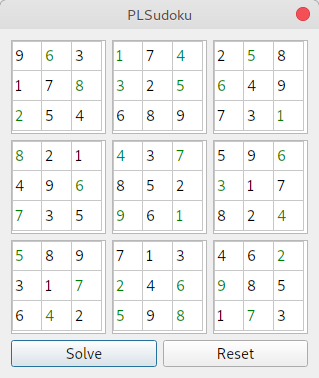
\includegraphics[scale=0.45]{../img/screenshot}
	\label{fig:gui}
	\caption{Captura de pantalla de la interfaz gráfica creada.}
\end{figure}

Es notable la rapidez con la que Prolog resuelve el puzzle dado que no fue detectado ningún tipo de retraso durante las pruebas.

\end{document}